%In coverage based evolutionary fuzz testing, every input that triggers new behavior will be added to an interesting seed queue which will then be used as the template file for next mutation. While as the testing goes on, more and more new seed files will be added into the queue, especially for large-scale modern software, the size of the queue can quickly reach a very large number. Obviously, mutating for every test case in the queue will last for a long time, so, in order to find more bugs or maximize the coverage in a time budget, we should introduce search strategy to prioritize the test cases.

As mentioned before, the size of the seed queue of coverage based evolutionary fuzz testing will quickly reach a large number when testing large-scale modern software. Mutating for each seed file will last for long time which will reduce the efficiency when given a time budget. 

We realized that different seed files in the queue have different power of finding new paths. For example in Figure~\ref{motivate-example}, suppose the state space of a program is modeled as a two-dimensional space, and each input that triggers new behavior will be mapped to a specific point in the space. The fuzz test starts from an initial seed which is marked as red in this figure. The mutation results of this initial seed covers the black points as well as seed A and seed B. Then, in evolutionary fuzz testing, a test case will be picked up from such new paths as the seed file for next round of mutation. 

Consider the choice between seed A and B in this figure, the \emph{distance}(eg. Euclidean Distance) from the initial seed file to A is much shorter than B, which, in other words, means that A is more \textbf{\textit{similar}} with the initial seed file than B. So choosing A as the next seed file to mutate will only trigger two new paths as most of the coverage are is (the blue area) overlapped with what of the initial seed file (the gray area). However, because seed B has a longer distance from the initial seed than seed A, and the coverage area of B (the brown area) will have less overlap with that of initial seed file than A. So choosing seed B will trigger more new behaviors than selecting seed A.


Based on this insight, we proposed a test case prioritization method based on \emph{distance}. Our method leverages three distance measures in regression testing, i.e. \textit{Euclidean distance}, \textit{Cosine similarity} and \textit{Jaccard index}, as the classification metrics for test case prioritization. Each test case in the seed queue will be assigned with a \emph{weight} value after being mapped as a vector from input space to state space. The \emph{weigth} value is utilized as the criteria to determine which seed file should be scheduled as next seed through a global optimum solution.

In the following sections, we firstly introduce these three similarity measures and then explain how a test case is mapped as a numerical vector. At last, the seed prioritization algorithm is described in detail as well as the distance calculation of the test case vectors.

\begin{figure}
\centering
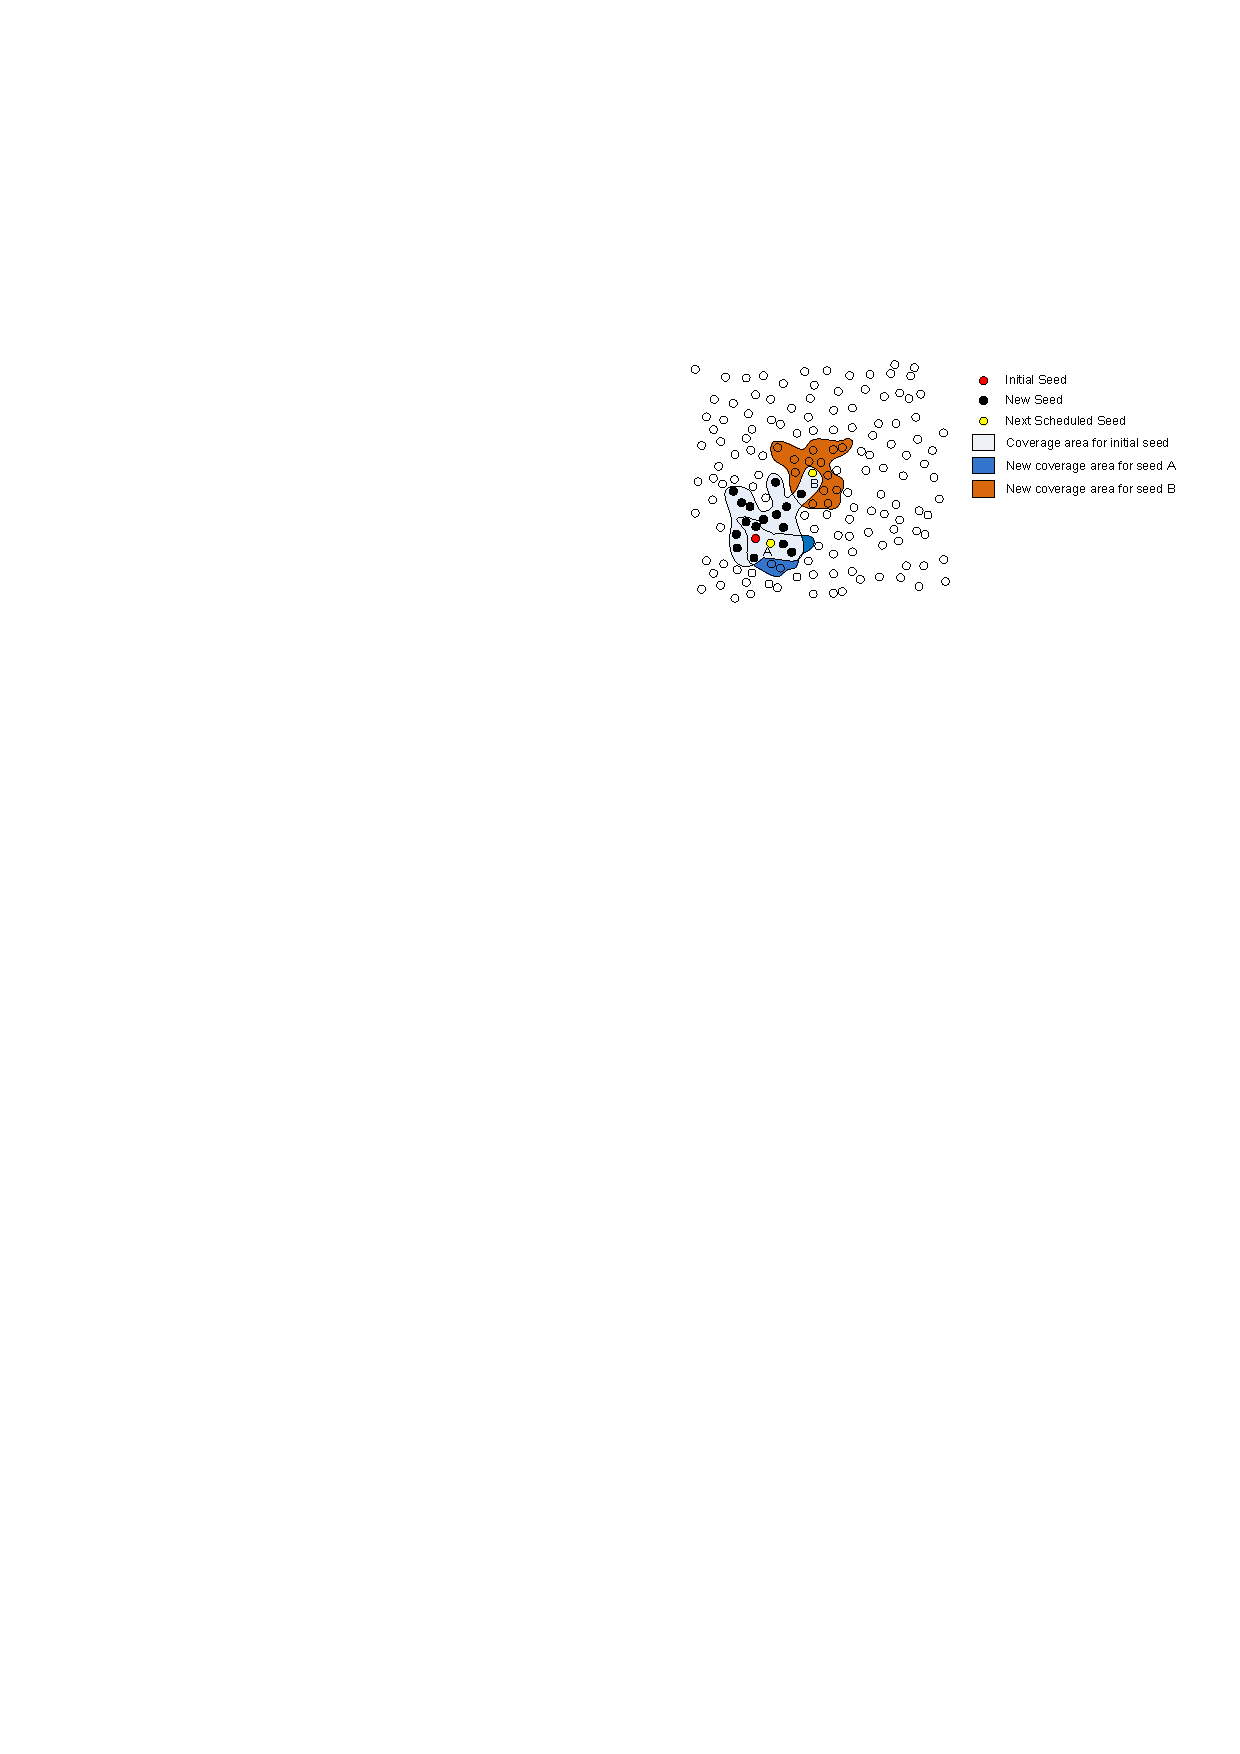
\includegraphics[width=0.7\textwidth]{figures/motivate-example.pdf} 
\caption{An motivate example.}\label{motivate-example}
\end{figure}

\subsection{Distance Metrics}
For two vectors $\mathit{X} = (x_1, x_2, \cdots, x_N)$ and $\mathit{Y} = (y_1, y_2, \cdots, y_N)$, the corresponding similarity metrics for \textit{Euclidean Distance}, \textit{Cosine Similarity} and \textit{Jaccard Index} are listed as follows.

\begin{enumerate}
\item Euclidean Distance (EU)

The Euclidean Distance between two vectors is defined as follows:
\begin{center}
$EU(\mathit{X}, \mathit{Y}) = \displaystyle \sqrt{\sum_{i=1}^{N} (x_i-y_i)^2}$
\end{center}


\item Cosine Similarity (CS)

The consine similarity between $\mathit{X}$ and $\mathit{Y}$ is defined as follows:

\begin{center}
$CS(\mathit{X}, \mathit{Y}) = \displaystyle \sqrt{\frac{\mathit{X}^T \cdot \mathit{Y}} {\| \mathit{X} \|\| \mathit{Y} \|}}$
\end{center}
where $\mathit{X}^T$ is a transposition of vector $\mathit{X}$ and $\| \mathit{X}\|$ is the Euclidean Distance of
vector $\mathit{X}$. Similarly, $\|\mathit{Y}\|$ is the Euclidean norm of vector $\mathit{Y}$. In essence, \textit{CS} is the cosine of the angle between $\mathbb{X}$ and $\mathit{Y}$ in the N-dimensional space. For Cosine similarly, the corresponding distance is defined as:

\begin{center}
$D(\mathit{X},\mathit{Y}) = 1 - CS(\mathit{X},\mathit{Y})$
\end{center}

\item Jaccard Index (JI)

The Jaccard Index between $\mathit{X}$ and $\mathit{Y}$ is defined as follows:

\begin{center}
$JI(\mathit{X}, \mathit{Y}) = \displaystyle \frac{\mathit{X} \cdot \mathit{Y}}{\mathit{X} \cdot \mathit{Y}+\omega(\|\mathit{X}\|^2+\|\mathit{Y}\|^2-2(\mathit{X} \cdot \mathit{Y}))}$
\end{center}

where $\mathit{X} \cdot \mathit{Y}$ is the inner product of $\mathit{X}$ and $\mathit{Y}$. 
When $\omega$ is equal to 1, the above formula is called Jaccard Index and its corresponding distance is defined as follows:

\begin{center}
$D(\mathit{X},\mathit{Y}) = 1 - JI(\mathit{X},\mathit{Y})$
\end{center}

\end{enumerate}

\subsection{Prioritizition Method}
In order to measure the distances between test cases, all the test cases should be mapped to vector space. 
The mapping can be performed both from input space and state space. However, mapping from input space cannot reflect the real relationship between test cases when considering the behavior of the target program. For example, as shown in Figure~\ref{distance-illusion}, multiple different inputs can steer the program to execute the same path. Specifically, considering the three test cases namely \texttt{A.jpeg}, \texttt{B.jpeg} and \texttt{C.jpeg} in this figure, suppose the corresponding contents are shown as follows:
\\
\\
\indent\texttt{A.jpeg}: \texttt{$\backslash$xFF$\backslash$xD8$\backslash$xAA$\backslash$xBB$\backslash$xCC$\backslash$xDD}

\texttt{B.jpeg}: \texttt{$\backslash$xFF$\backslash$xD8$\backslash$xDD$\backslash$xCC$\backslash$xBB$\backslash$xAA}

\texttt{C.jpeg}: \texttt{$\backslash$xFE$\backslash$xD8$\backslash$xAA$\backslash$xBB$\backslash$xCC$\backslash$xDD}
\\

\indent Obviously, if we calculate the \textit{Euclidean Distance} between these three files based from input space, $ED_{AB}$ will be greater than $ED_{AC}$ because there are more different bytes between \texttt{A.jpeg} and \texttt{B.jpeg} than that of \texttt{A.jpeg} and \texttt{C.jpeg}. This means \texttt{A.jpeg} and \texttt{C.jpeg} are more similar (as shown in Figure~\ref{distance-illusion}) from the viewpoint in the input space. 
However, for most of the JPEG process programs, \texttt{A.jpeg} and \texttt{B.jpeg} will execute the same path. However, \texttt{C.jpeg} will execute another path because \texttt{C.jpeg} is an illegal JPEG file (bad magic number). So from the viewpoint of program, \texttt{A.jpeg} and \texttt{B.jpeg} are more similar than \texttt{A.jpeg} and \texttt{C.jpeg} even though \texttt{A.jpeg} and \texttt{C.jpeg} have only one bit difference. 
Since our objective is to maximize the coverage in the state space, so we choose to map all the test cases from the state space to numeric vectors to calculate the distance.

In \cite{wang2015similarity} all test cases are represented as a branch coverage vector $\mathit{V}=(v_1, v_2, \cdots, v_N)$, where $v_i$ is 0 means the branch is covered, otherwise 1. 
However, different test cases can affect different branches, so the mapped vectors may have different lengths which cannot be used directly for distance calculation. Meanwhile, it will be very difficult to construct such vectors because it is hard to obtain all the branches and list them orderly in each vector to avoid obfuscation between vectors. 
In AFL \cite{online:afl}, the execution path information of each test case is recorded into a \emph{Bitmap}. This \emph{Bitmap} is then used to determine whether a test case triggers new behaviors by comparing it with a global one. And the \emph{Bitmap} in AFL contains enough information to reflect the characteristics of a test case from the viewpoint of the state space. 
So we selected the \emph{Bitmap} used in AFL as our mapped vector to mitigate the costly mapping as the list of ordered branches like \cite{wang2015similarity}.

\begin{figure}
\centering
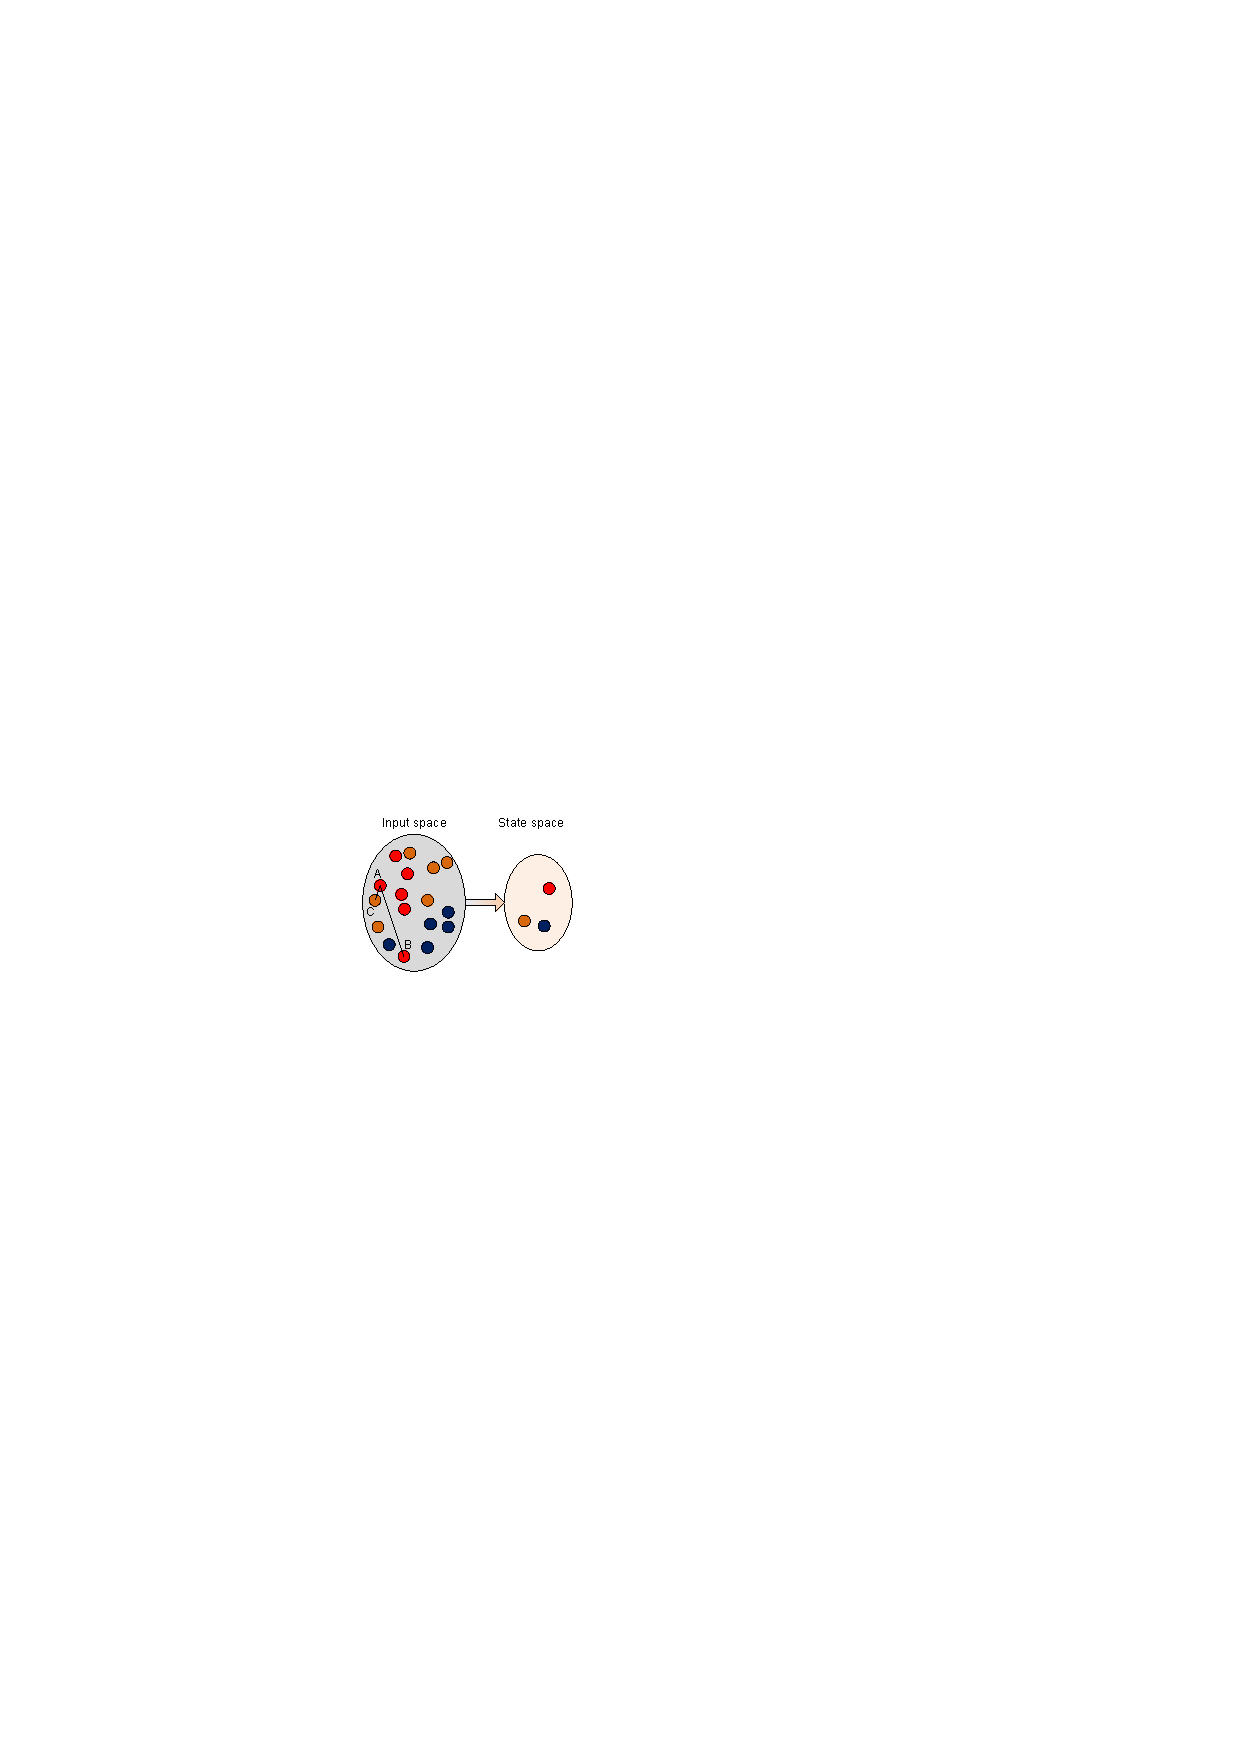
\includegraphics[width=0.5\textwidth]{figures/distance-illusion.pdf} 
\caption{An illusion for distance.}\label{distance-illusion}
\end{figure}

Based on the mapped bitmap vectors, the test case queue in the fuzzer is enhanced by assigning each test case with weight $W$ which is obtained from the distance between every two test cases. Whenever a new seed file is found, the distance between this seed file and all the other files in the queue will be measured to calculate $W$. And meanwhile, the weight of all the other files in the queue will be updated according to the distance to the new seed file. 

Rather than selecting the seed file that has the longest distance to the current seed file which is only a \emph{local optimum solution}, our search method selects the file that takes the longest average distance from all the other test cases as the next seed file. By doing this, we can achieve the \emph{global optimum solution} for this searching problem. The weight $W$ for $t_k$ is defined as follows:

\begin{center}
$W_k = \displaystyle\frac{1}{N} \sum_{i=0}^{N} D(t_i, t_k)$
\end{center}

where $D(t_i, t_k)$ denotes the distance between $t_i$ and $t_k$ based on the three distance measures mentioned before, and $N$ is the size of the test case queue. 